\documentclass[
]{beamer}

\usepackage[english]{babel}
\usepackage[utf8]{inputenc}
\usepackage[T1]{fontenc}
\usepackage{csquotes}
\usepackage{expl3,biblatex}
\addbibresource{main.bib}
\usepackage{booktabs}
\usetheme[
  workplace=fi,
  ]{MU}
\usepackage{textalpha}
\usepackage{subfigure}
\usepackage{wrapfig}
\usepackage{tikz}
\usepackage{appendixnumberbeamer}

\title[Visualization of partial charges in Mol*]{Modern visualization of partial atomic charges in Mol*}
\subtitle[Short Presentation Subtitle]{Bachelor's thesis defense}
\author[D. Tichý]{Dominik Tichý\texorpdfstring{\\}{, }Supervisor: RNDr. Tomáš Raček, Ph.D.}
\institute[FI MU]{Faculty of Informatics, Masaryk University}
\date{June 30, 2023}
\subject{Presentation Subject}
\keywords{the, presentation, keywords}
\begin{document}

\begin{frame}[plain]
  \maketitle
\end{frame}

\begin{wrapfigure}{r}{0.5\textwidth}
  \vspace{55pt}
  \hspace{45pt}
  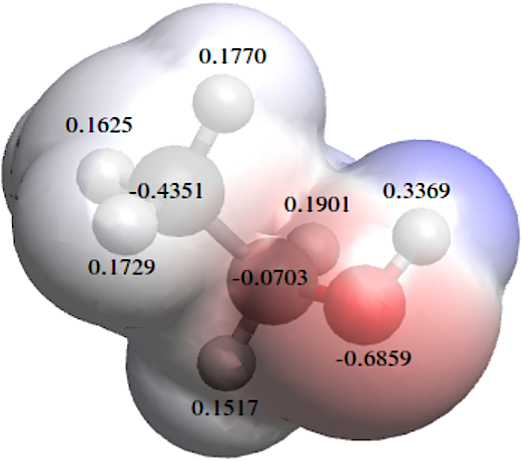
\includegraphics[height=3cm]{images/charges-numbers.png}
\end{wrapfigure}

\begin{frame}{Partial atomic charges}
  \begin{itemize}
    \item real numbers describing the distribution of electron density among atoms in a molecule
    \item applications:
    \begin{itemize}
      \item molecular docking
      \item pharmacophore modeling
      \item molecular dynamics simulations
    \end{itemize}
      \item calculation methods:
    \begin{itemize}
      \item quantum mechanics - extremely slow
      \item empirical methods - much faster with slight cost to accuracy
    \end{itemize}
  \end{itemize}
\end{frame}

\begin{frame}{Empirical methods -- implementations}
  \begin{itemize}
    \item web applications for calculating partial atomic charges:
    \begin{itemize}
      \item Atomic Charge Calculator~II (ACC~II) \footfullcite{racek2020atomic}
      \item αCharges (AlphaCharges) \footfullcite{schindler2023acharges2}
    \end{itemize}
    \item developed by the Structural Bioinformatics research group at the National Centre for Biomolecular Research 
  \end{itemize}
\end{frame}

\begin{frame}{Motivation \& Thesis goals}
  \textbf{Motivation:}
  \begin{itemize}
    \item both ACC~II and αCharges use the LiteMol Viewer
    \begin{itemize}
      \item no longer maintained $\rightarrow$ needs to be replaced
    \end{itemize}
    \item the Mol* Viewer is the modern replacement for LiteMol
    \begin{itemize}
      \item no support for partial atomic charges
    \end{itemize}
  \end{itemize}
  \vspace{10pt}
  \textbf{Goals:}
  \begin{enumerate}
    \item study the necessary theory on partial atomic charges
    \item extend Mol* Viewer to support partial charge visualization
    \item integrate the updated Mol* Viewer into:
    \begin{itemize}
      \item ACC~II
      \item αCharges
    \end{itemize}
  \end{enumerate}
\end{frame}
    
\begin{frame}{Mol* extension}
  \begin{itemize}
    \item created mmCIF categories for storing partial atomic charges
    \item extended the Mol* Viewer to support visualization of charges
  \end{itemize}
  \begin{figure}
    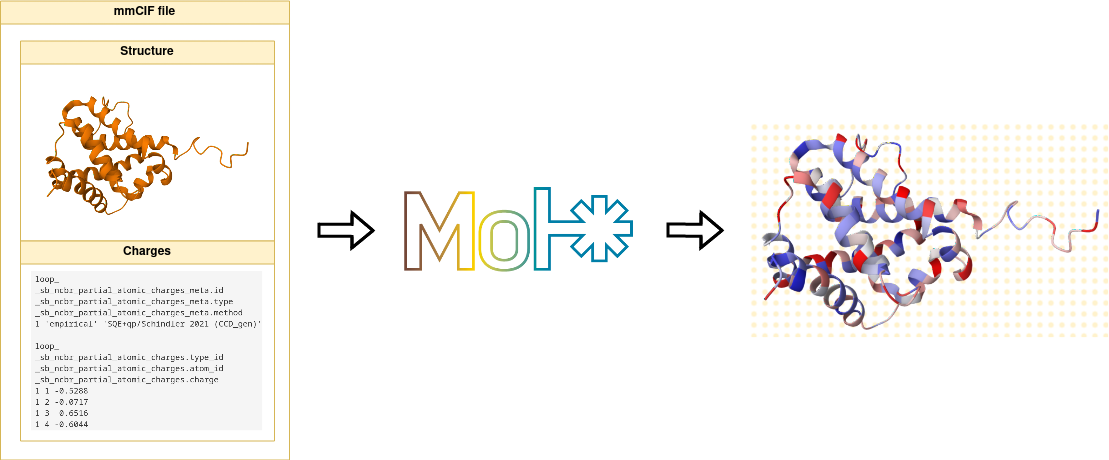
\includegraphics[width=\textwidth,keepaspectratio]{images/molstar-use-case.png}
  \end{figure}
\end{frame}

\section{Mol* extension}

\begin{frame}{}
  \begin{figure}
    \centering
    \subfigure[Ball and stick]{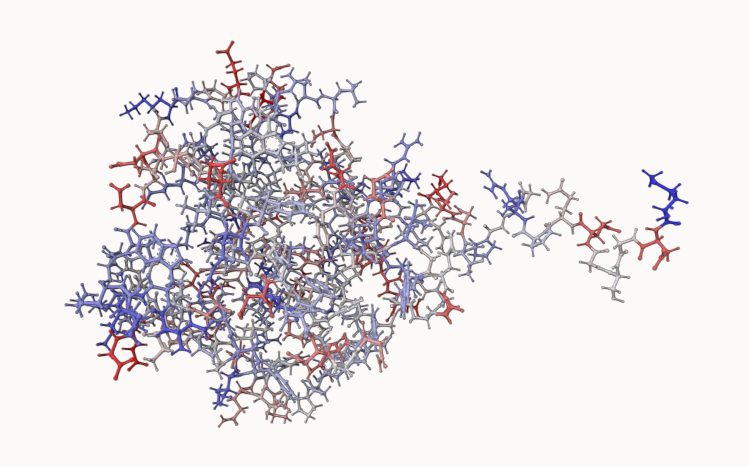
\includegraphics[width=0.45\textwidth]{images/1F162-bas.png}}
    \subfigure[Surface]{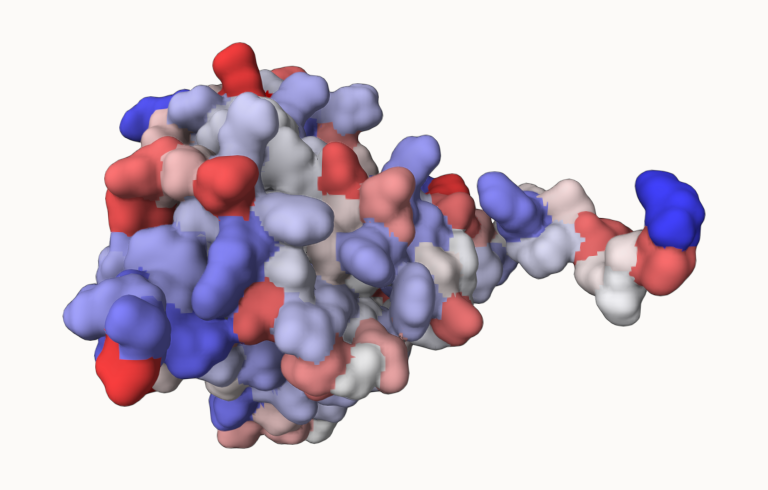
\includegraphics[width=0.45\textwidth]{images/1F16-surface.png}}
    \subfigure[Cartoon]{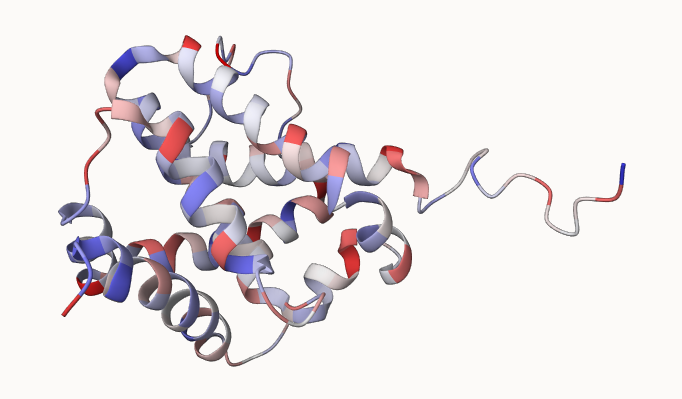
\includegraphics[width=0.45\textwidth]{images/1F16-cartoon.png}}
    \subfigure[Color gradients]{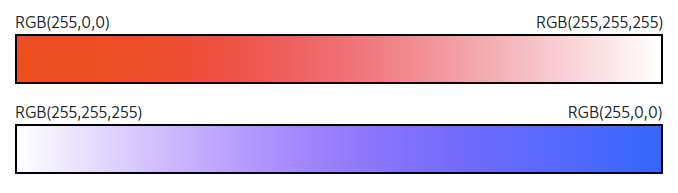
\includegraphics[width=0.45\textwidth]{images/color_gradients.png}}
  \end{figure}  
\end{frame}

\section[]{}

\begin{frame}{Integration of Mol* viewer into ACC~II}
  \begin{itemize}
    \item replaced the the LiteMol Viewer with the Mol* Viewer
    \item added support for multiple calculations on one request
  \end{itemize}
  \begin{figure}
    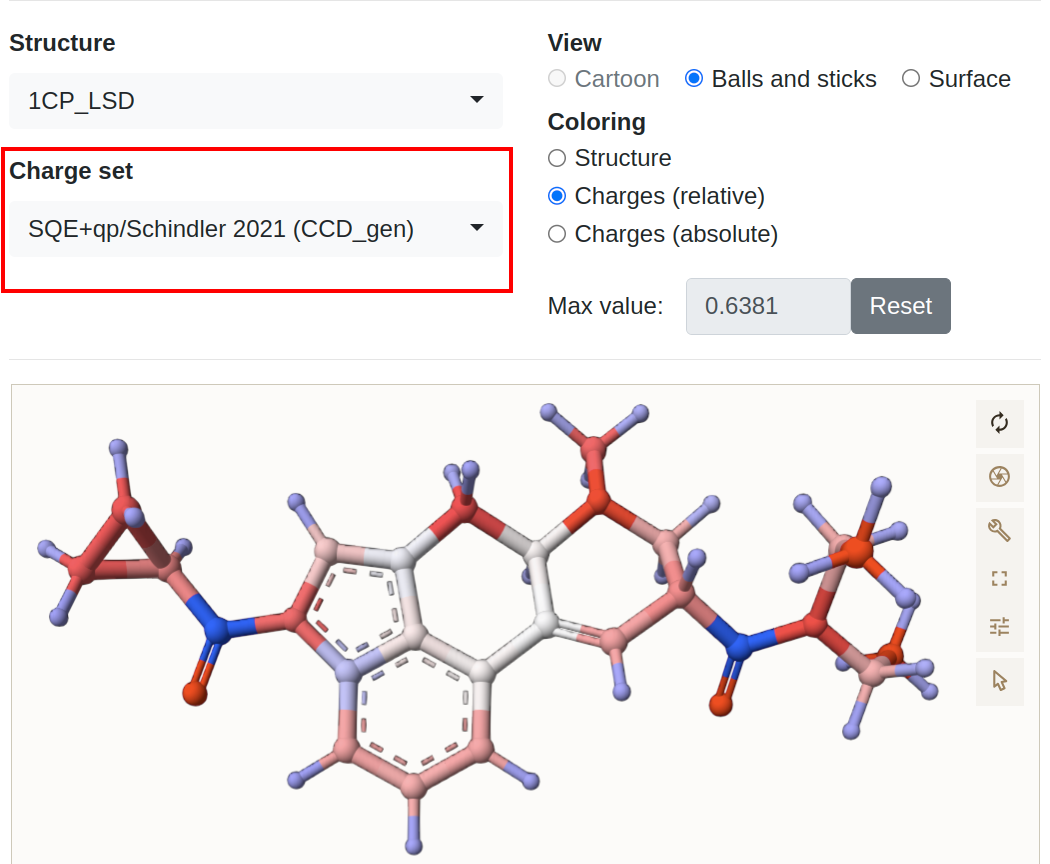
\includegraphics[width=1\textwidth,height=0.78\textheight,keepaspectratio]{images/acc2.png}
  \end{figure}
\end{frame}

\begin{frame}{Integration of Mol* viewer into αCharges}
  \begin{itemize}
    \item the Mol* Viewer is used for displaying the results
    \item added a page for describing problematic atoms
  \end{itemize}
  \begin{figure}
    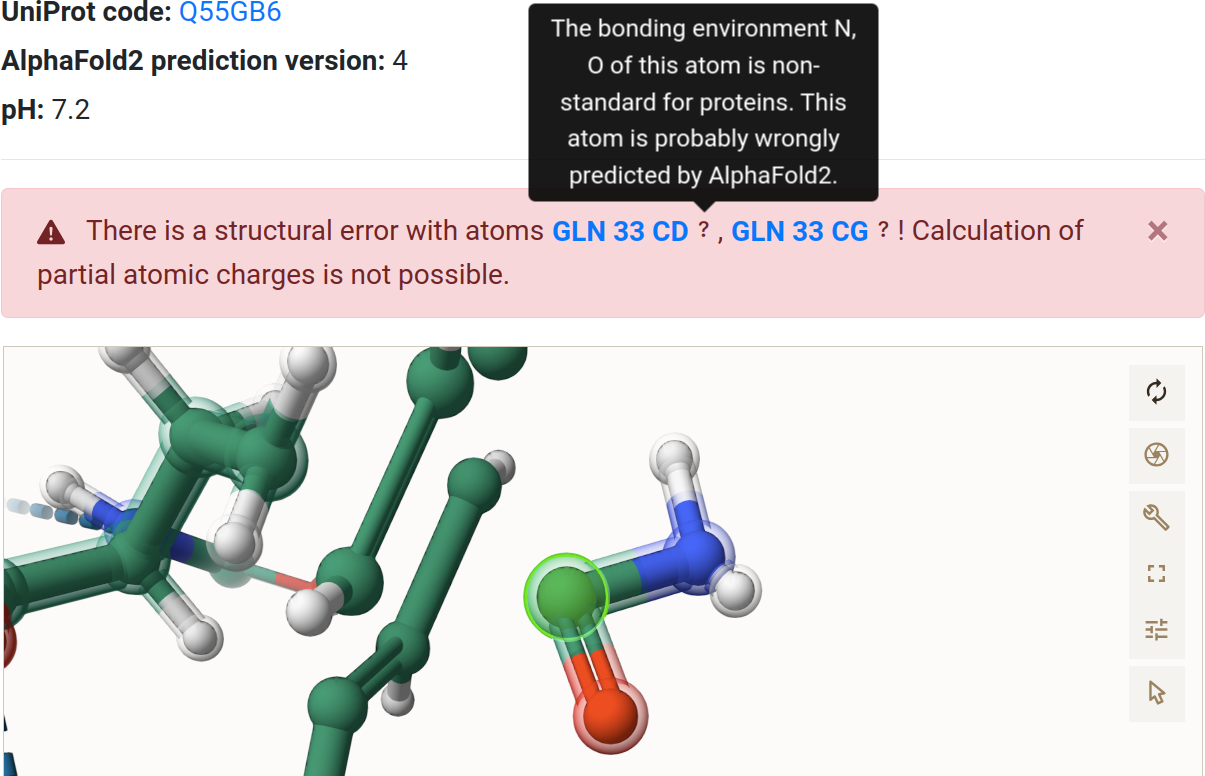
\includegraphics[width=1\textwidth,height=0.75\textheight,keepaspectratio]{images/focus.png}
  \end{figure}
  \end{frame}

\section[]{}

\begin{frame}{Nucleic Acids Research paper}
  \begin{itemize}
    \item the current impact factor of the journal is \textbf{19.160}
    \item \fullcite{schindler2023acharges}
  \end{itemize}
  \begin{figure}
    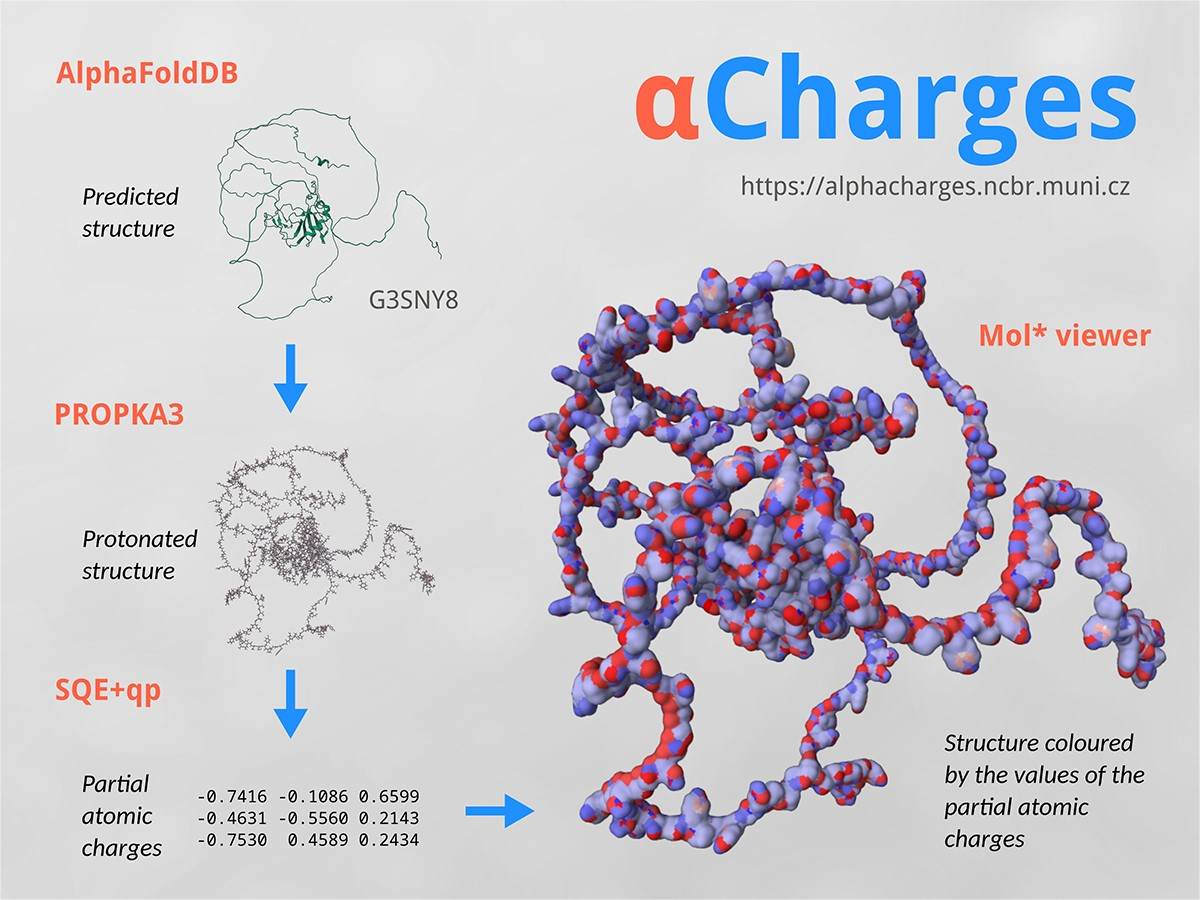
\includegraphics[width=0.6\textwidth,keepaspectratio]{images/alpha-charges-visualization.jpeg}
  \end{figure}
\end{frame}

\begin{frame}{Conclusion}
  \begin{itemize}
    \item created the Mol* extension for visualizing partial atomic charges
    \item integrated the updated Mol* Viewer into ACC~II and αCharges
    \item extended the capabilities of ACC~II to support multiple calculations on one request
    \item contributed with the work to the αCharges paper
  \end{itemize}
\end{frame}

\begin{frame}[plain,noframenumbering]
  \tikz[remember picture,overlay] \node[opacity=1,inner sep=0pt] at (current page.center){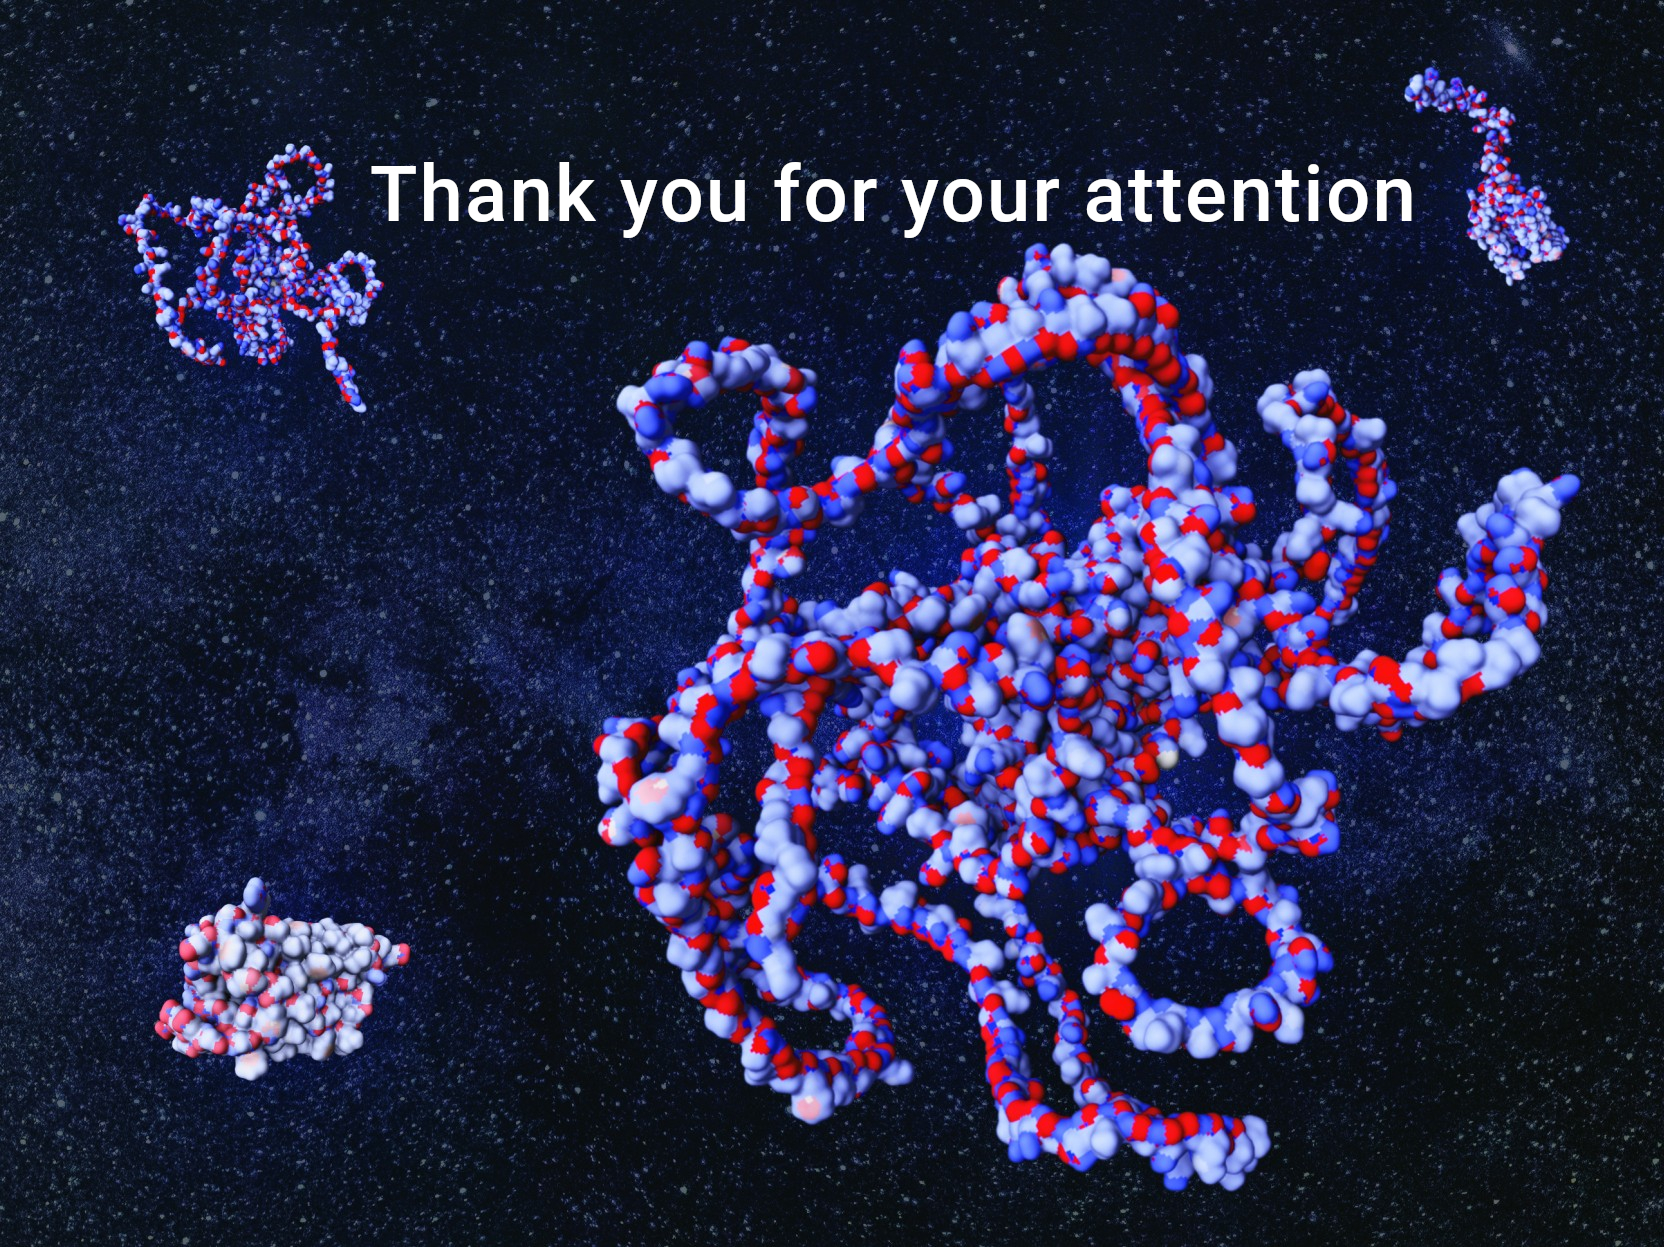
\includegraphics[width=\paperwidth,height=\paperheight]{images/thank-you.jpg}};
  \clearpage
\end{frame}

\appendix

\section{Otázky oponenta}

\subsection[1]{1}

\begin{frame}
  \begin{block}{Otázky oponenta 1}
    Proč jste pro vývoj Mol* pluginu zvolil Vite build tool? Zvažoval jste i jiné alternativy?
  \end{block}
  \begin{itemize}
    \item Mol* používá Webpack
    \item Vite poskytuje rychlejší development server a optimalizované produkční buildy
  \end{itemize}
\end{frame}

\begin{frame}
  \begin{figure}
    \includegraphics[width=0.7\textwidth,height=\textheight,keepaspectratio]{images/build_tools_experience_ranking.png}
    \caption{Retence build nástrojů v průzkumu State of JS 2022
      \footnote{\url{https://2022.stateofjs.com}}
    }
  \end{figure}
\end{frame}

\subsection[2]{2}

\begin{frame}
  \begin{block}{Otázky oponenta 2}
    V jakých formátech je možno načíst náboje do Mol*?
  \end{block}
  \begin{itemize}
    \item Mol* Viewer umožňuje načíst náboje pouze v mmCIF formátu
    \item je možné přidat podporu pro další formáty, které mají datová pole pro náboje
    \begin{itemize}
      \item MOL2
      \item PQR
    \end{itemize}
    \item lze také oddělit strukturu od nábojů a načítat je zvlášť
    \begin{itemize}
      \item vyžadovalo by to vytvořit nástroje na importování nábojů 
      \item tento přístup byl použit v rozšíření LiteMol Vieweru
    \end{itemize}
  \end{itemize}
\end{frame}

\subsection[3]{3}

\begin{frame}
  \begin{block}{Otázky oponenta 3}
    Jste schopen využít funkcionalitu pro vizualizaci nábojů v Mol* i pro více přiložených molekul? Pokud ano, mohl byste to ukázat na příkladu? Např. podle nábojů obarvit a přiložit PIN proteiny, které jsou využity jako use case na webu αCharges?
  \end{block}
  \begin{itemize}
    \item ano, struktury s vypočítanými náboji z αCharges lze nahrát do Mol* a v něm provést přiložení
  \end{itemize}
\end{frame}

\begin{frame}
  \begin{figure}
    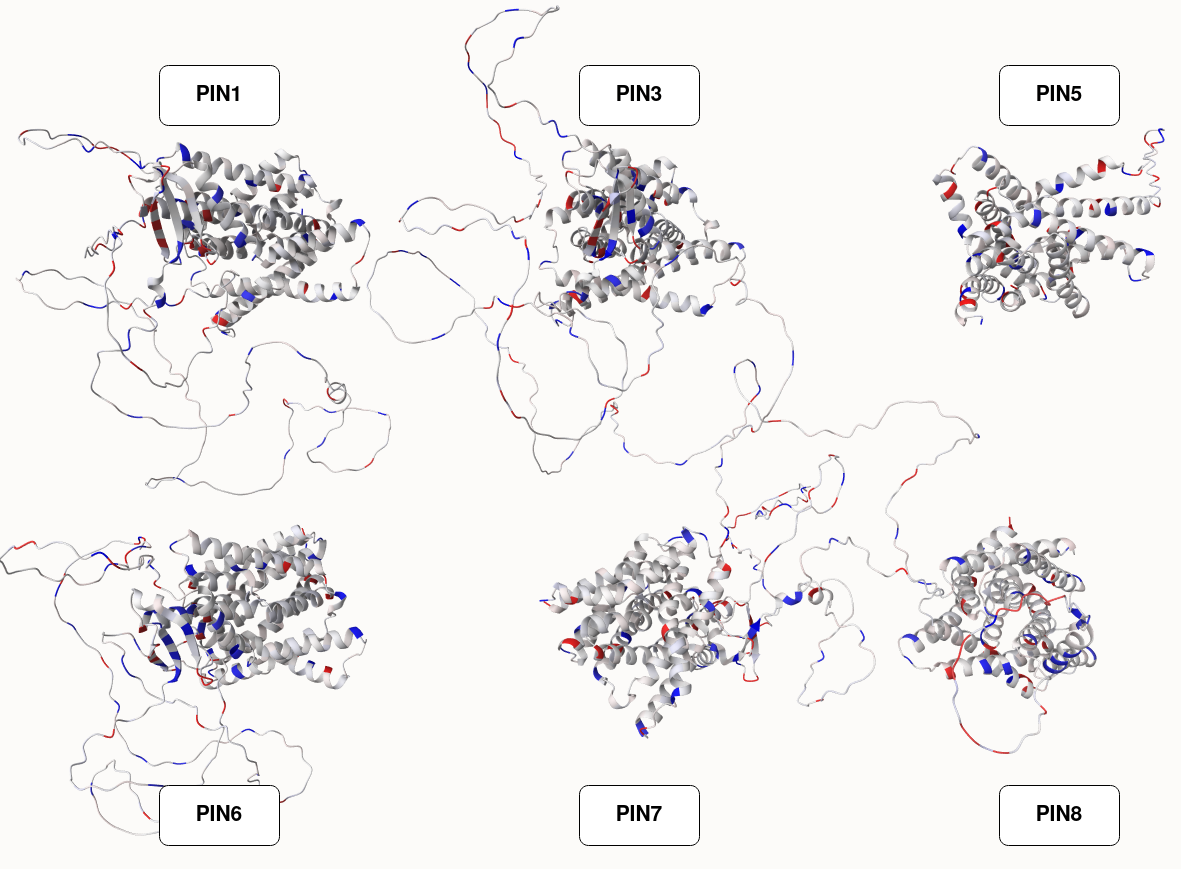
\includegraphics[width=1\textwidth,height=\textheight,keepaspectratio]{images/pins2.png}
  \end{figure}
\end{frame}

\subsection[4]{4}

\begin{frame}
  \begin{block}{Otázky oponenta 4}
    Bylo by možno do budoucna podle nábojů obarvit i jiné objekty než atomy, elementy sekundární struktury nebo povrchy atomů - např. póry a kanály v proteinech? A pokud ano, jak pracné by to bylo?
  \end{block}
  \begin{itemize}
    \item ano, je to možné
    \item časový odhad: pár týdnů
    % \item obarvování používá Location objekt, podle kterého se určí jakou barvu obarvit daný prvek reprezentace (např. atom, vazbu)
    % \item bylo by nutné vytvořit novou 3D reprezentaci (např. pro póry, kanály)
    % \begin{itemize}
    %   \item tato reprezentace by musela poskytnout Location objekty pro každou část póru/kanálu
    % \end{itemize}
  \end{itemize}
\end{frame}

\section[Bonus slides]{Bonus slides}

\subsection[mmCIF categories]{mmCIF categories}

\begin{frame}
  \begin{figure}
    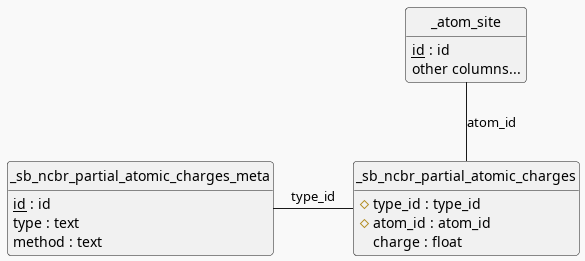
\includegraphics[width=0.8\textwidth,keepaspectratio]{images/mmcif_erd.png}
    \caption{Diagram of the custom mmCIF categories}
  \end{figure}
\end{frame}

\subsection[PINS]{PINS}

\begin{frame}
  \begin{figure}
    \includegraphics[width=1\textwidth,height=\textheight,keepaspectratio]{images/alpha-charges-examples.png}
  \end{figure}
\end{frame}

\begin{frame}
  \begin{figure}
    \includegraphics[width=1\textwidth,height=\textheight,keepaspectratio]{images/pin1-download.png}
  \end{figure}
\end{frame}

\begin{frame}
  \begin{figure}
    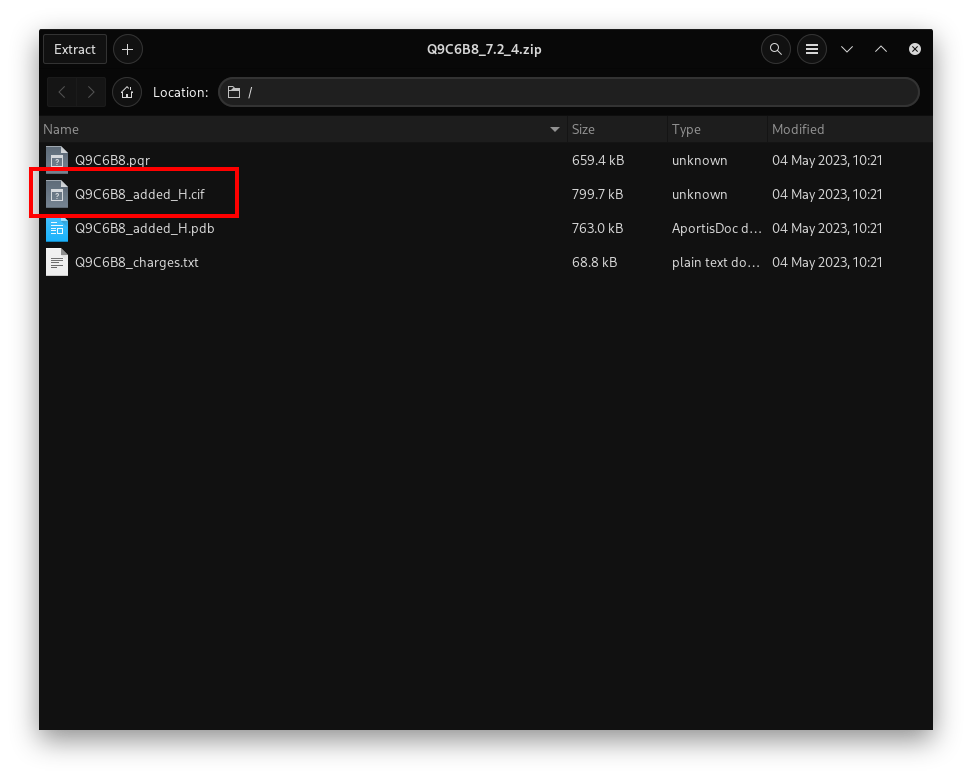
\includegraphics[width=1\textwidth,height=\textheight,keepaspectratio]{images/folder.png}
  \end{figure}
\end{frame}

\begin{frame}
  \begin{figure}
    \includegraphics[width=1\textwidth,height=\textheight,keepaspectratio]{images/pins-folder.png}
  \end{figure}
\end{frame}

\begin{frame}
  \begin{figure}
    \includegraphics[width=1\textwidth,height=\textheight,keepaspectratio]{images/pins1.png}
  \end{figure}
\end{frame}

\begin{frame}
  \begin{figure}
    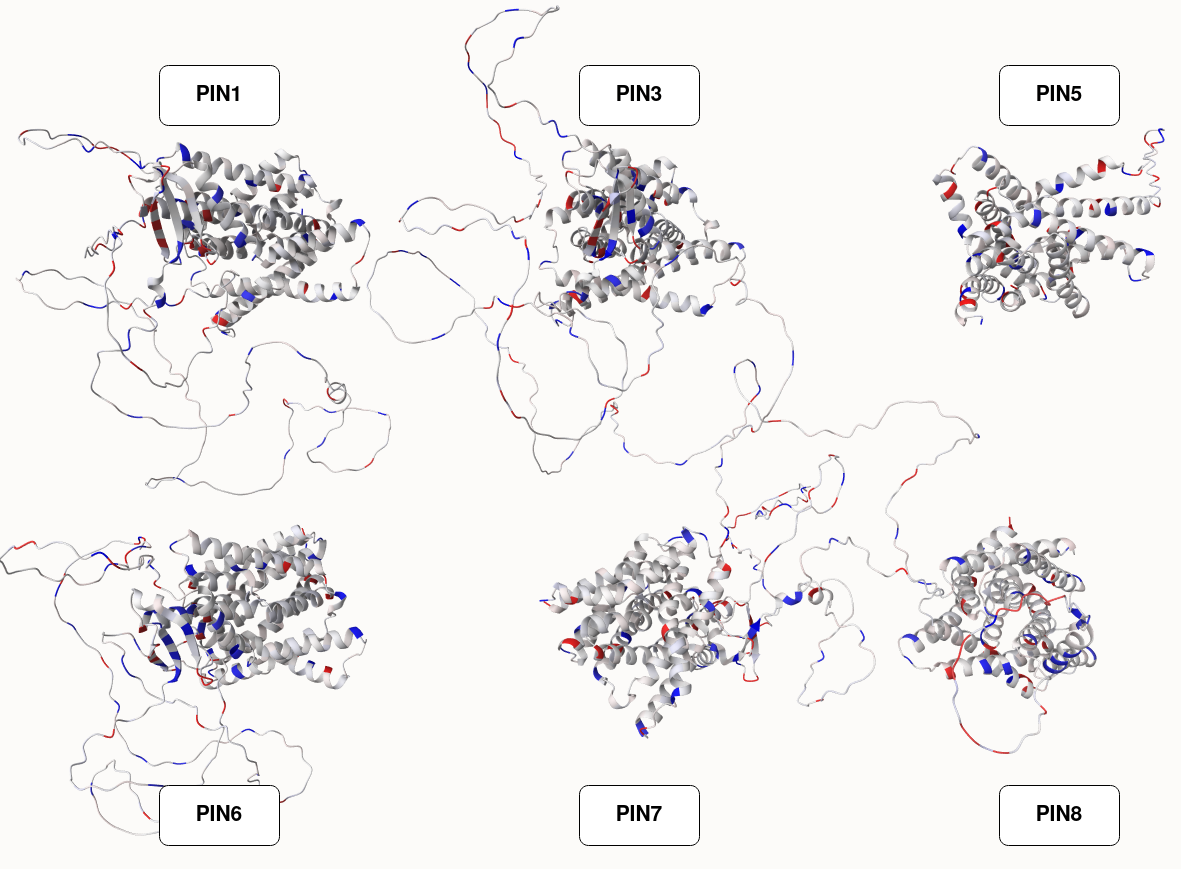
\includegraphics[width=1\textwidth,height=\textheight,keepaspectratio]{images/pins2.png}
  \end{figure}
\end{frame}

\subsection[Vite]{Vite}

\begin{frame}
  \begin{itemize}
    \item \textbf{Fast start}
    \begin{itemize}
        \item prebundles dependencies using \textit{esbuild}
        \item serves source code with native ESM modules
    \end{itemize}
    \item \textbf{Fast updates}
    \begin{itemize}
        \item HMR is performed over native ESM
        \item leverages HTTP headers to speed up full page reloads
    \end{itemize}
\end{itemize}
\end{frame}


\begin{frame}
  \begin{figure}
    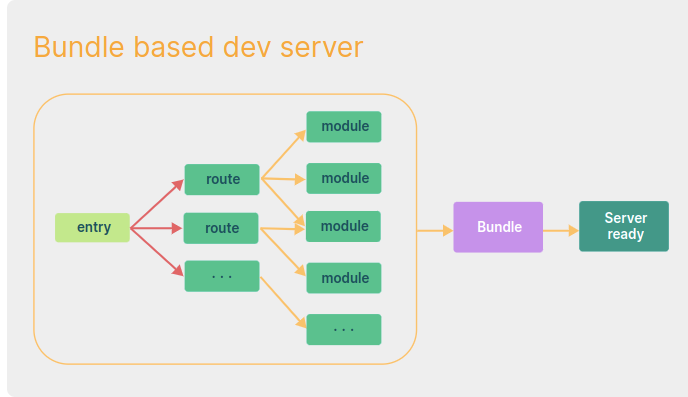
\includegraphics[width=0.8\textwidth,height=\textheight,keepaspectratio]{images/bundle_dev_server.png}
    \caption{Bundle-based development server
    \footnote{\url{https://vitejs.dev/guide/why.html}}
  }
  \end{figure}
\end{frame}

\begin{frame}
  \begin{figure}
    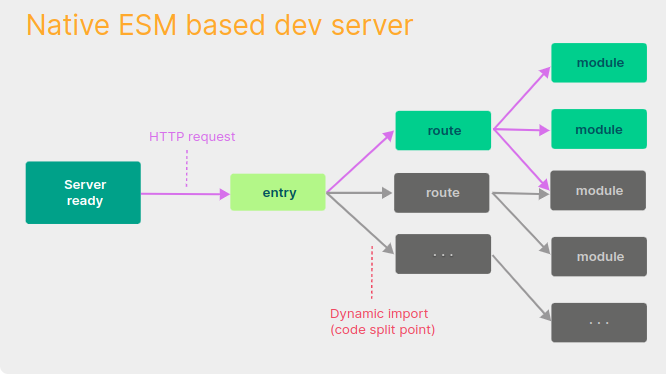
\includegraphics[width=0.8\textwidth,height=\textheight,keepaspectratio]{images/native_esm_dev_server.png}
    \caption{Native ESM module development server
    \footnote{\url{https://vitejs.dev/guide/why.html}}
  }
  \end{figure}
\end{frame}

\makeoutro
\addtocounter{framenumber}{-1}

\end{document}
